\documentclass{article}

\usepackage{repsty}

\newcommand{\nb}{{n_b}}

\newcommand{\uvec}[1]{\boldsymbol{\hat{#1}}}
\newcommand{\abs}[1]{\vert#1\vert}
\newcommand{\proj}[2]{\pi_{\uvec{#2}}\vec{#1}}

\newcommand{\Dw}{\Delta\omega}
\newcommand{\ii}{\imath}
\begin{document}

\section{Projection of polarization}
The polarization of the beam is the sum of the spins of the particles in it. We measure the projection of the polarization on the $y$-axis:
\begin{align}
	\vec{P} &= \sum_{i=1}^\nb \vec{s}, \notag\\
	\proj{s}{y} &\equiv \uvec{y}\cdot\vec{s} = \abs{\vec{s}}\cos\Theta, \notag\\
	\proj{P}{y} &= \sum_i \proj{s_i}{y} = \abs{\vec{s}}\sum_i \cos\Theta_i, \label{eq:SumSpins}
\intertext{where the particles' phases and oscillation frequencies are randomly distributed:}
	\Theta_i &= \omega_i\cdot t + \phi_i,~ f(\phi_i),~g(\omega_i).\notag
\end{align}

The phase $\Theta_i$ is a random variable, hence $\proj{P}{y}$ is a sum of random variables; this sum is distributed normally, with expectation $\Xpct{\proj{P}{y}}[t] = \abs{\vec{s}}\cdot\nb\cdot \int_\infty\cos\theta\cdot f(\theta|t)\td\theta$.

\section{Simulation}
\newcommand{\Norm}{\mathcal{N}}
\newcommand{\dy}{\Delta\gamma}
\newcommand{\ycoef}{h}
\newcommand{\wcoef}{G}
\newcommand{\dwcoef}{g}
\newcommand{\vp}[2]{{#1}\cdot 10^{#2} }
In the simulation, the following model was assumed:\\
\begin{minipage}{.5\textwidth}
	\begin{align*}
		\dy &\sim \Norm(0, \SD{\dy}), \\
		\SD{\dy}(t) &= \SD{\dy}(0) + \ycoef\cdot t, \\
		\omega_i &= \omega_0 + \wcoef\cdot \dy_i^2, \\
		\phi &\sim \Norm(\phi_0, \SD{\phi}).
	\end{align*}
\end{minipage}
\begin{minipage}{.5\textwidth}
	\begin{tabular}{clr}
		  Parameter   & Value            &          Dimension \\ \hline
		$\SD{\dy}(0)$ & $\vp{1}{-3}$     &  \\
		  $\ycoef$    & $\vp{5}{-6}$     &   $\sfrac{1}{sec}$ \\
		 $\omega_0$   & $3$              & $\sfrac{rad}{sec}$ \\
		  $\wcoef$    & $\vp{1}{3}$      & $\sfrac{rad}{sec}$ \\
		  $\phi_0$    & $\sfrac{\pi}{2}$ &  \\
		 $\SD{\phi}$  & $\vp{2}{-2}$     &              $rad$ \\ \hline
	\end{tabular}
\end{minipage}


\subsection{Constant $\SD{\dy}(t=0)$}
Given unchanging distributions of the beam particles' phase and oscillation frequency presented in Figure~\ref{fig:PSdist_cDy} (sampled once at time $=0$), the resulting polarization signal, computed according to eq.~\eqref{eq:SumSpins}, has the form shown in Figure~\ref{fig:Sgl_cDyPhys}.
\begin{figure}[h]
	\begin{subfigure}[b]{.45\textwidth}
		\centering
		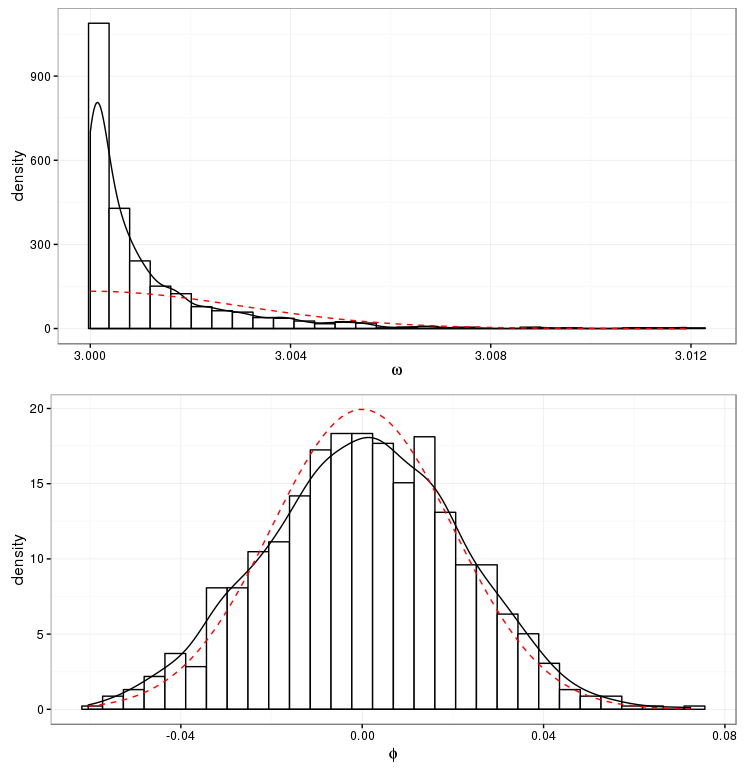
\includegraphics[scale=.5]{../img/PS_dist}
		\caption{Phase space distributions.\label{fig:PSdist_cDy}}
	\end{subfigure}~~~~~~~~
	\begin{subfigure}[b]{.45\textwidth}
		\centering
		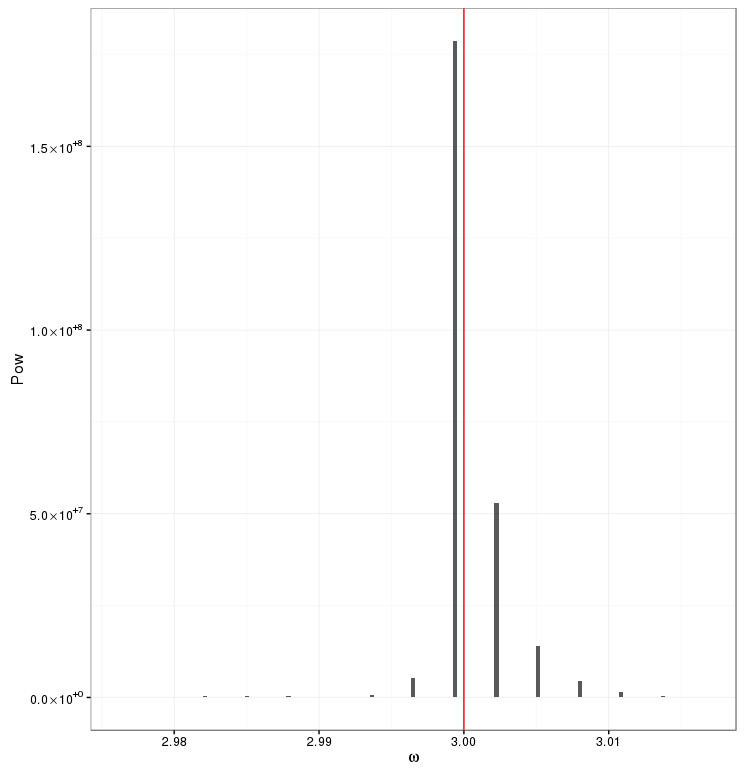
\includegraphics[scale=.5]{../img/Spec_PhysDistros}
		\caption{Power spectral density plot.\label{fig:PSD_cDyPhys}}
	\end{subfigure}
	\caption{Distributions and power spectra.}
\end{figure}
\begin{figure}[h]
	\centering
	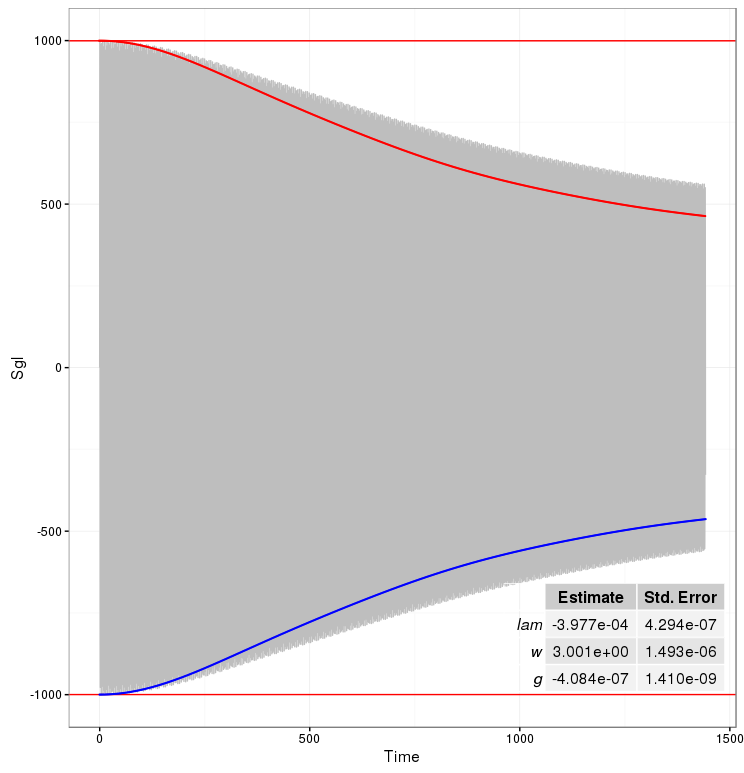
\includegraphics[scale=.6]{../img/Sgl_PhysDistros}
	\caption{Polarization signal in the case of constant phase space distributions. The black lines mark the measurements taken at the points $\sin(\omega_0\cdot t_n + \phi_0)=\pm 1$.\label{fig:Sgl_cDyPhys}}
\end{figure}

One can observe (the detailization in Figure~\ref{fig:Sgl_cDyPhys}) that the black lines, marking the measurements supposed to be at the peaks/valleys of the signal (the null envelope), fall in front of the actual extrema after a while, which suggests that the signal's oscillation frequency is greater than that of the synchronous particle, $\omega_0$. With that in mind, we fitted the function $f(t) = n_b\cdot\exp\bkt{\lambda t}\cdot\sin\bkt{(\omega+\dwcoef\cdot t)\cdot t + \phi_0}$ to the simulated data.

The model fit yielded an $\hat{\omega} \approx 3.001 \pm 1.535\cdot10^{-6}$, and a life-time $\hat{\tau}\approx 2600$ sec. The frequency growth factor, $g$, is estimated $\dwcoef < 0$, indicating a \emph{decreasing} oscillation frequency. The estimate of $g$ is statistically significant, with the t-value $\approx -270$; we note, however, that the used model is drastically misspecified,~\footnote{The first derivative of the signal's envelope falls much slower at the beginning.} which might be the cause of the contradiction between the supposed deceleration of oscillation, and the evidence of the computed envelope points. 

The signal's power spectrum (Figure~\ref{fig:PSD_cDyPhys}) mimics the particles' $\omega$ density distribution.

\subsection{Growing $\SD{\dy}(t)$}
In this simulation, we resampled the $(\omega,\phi)$ phase space at each measurement time. The effect of the growth of $\SD{\dy}$ can be observed not only in that the signal decays much more rapidly ($\hat{\tau}\approx 454$ sec), but also in the increase of $\Xpct{\hat{\omega}}$ from $3.001$ to $3.002$, caused by the appearance of a greater number of particles with higher frequencies.
\begin{figure}[h]
	\centering
	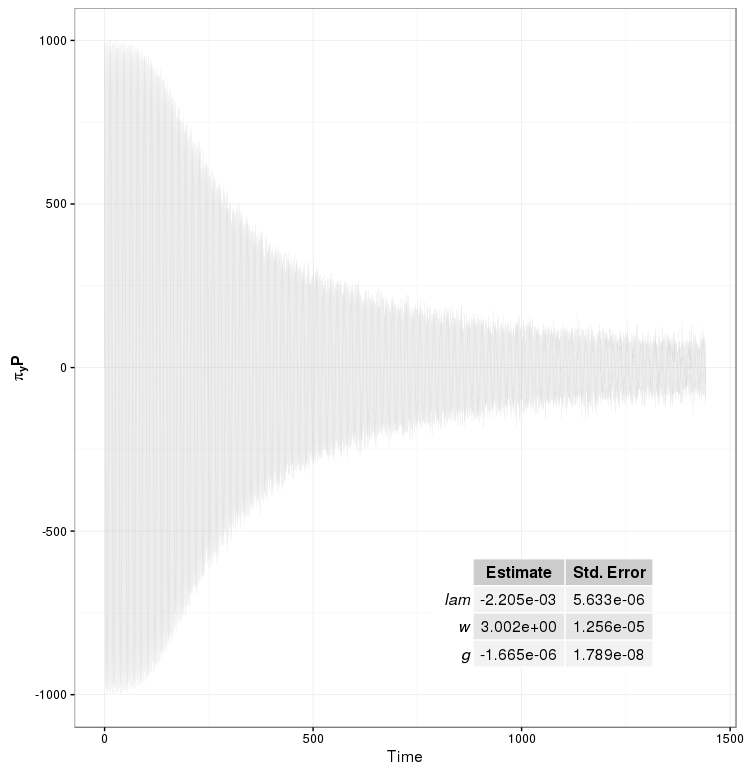
\includegraphics[scale=.6]{../img/Signal_Growing_Dgamma}
	\caption{Decoherence when $\SD{\dy}$ grows with time.}
\end{figure}

\subsection{Normally distributed $\omega$}
In this case (Figure~\ref{fig:Sgl_cDyNorm}) the shift in the signal peaks from the null envelope is unnoticeable (as further evidenced by the non-convergence of the model with a frequency growth factor). Any systematic deviation of $\Xpct{\hat{\omega}}$ is due to the asymmetry of the $\omega$ distribution, and therefore decreases with the number of particles used in modeling.
\begin{figure}[h]
	\begin{subfigure}{.5\textwidth}
		\centering
		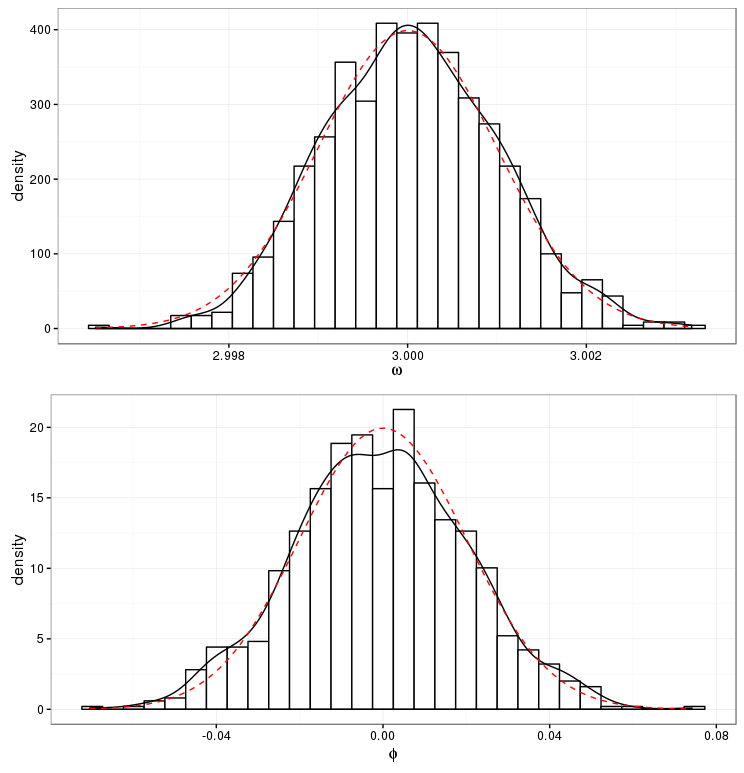
\includegraphics[scale=.5]{../img/PS_dist_Norm}
		\caption{Phase space distributions.}
	\end{subfigure}~
	\begin{subfigure}{.5\textwidth}
		\centering
		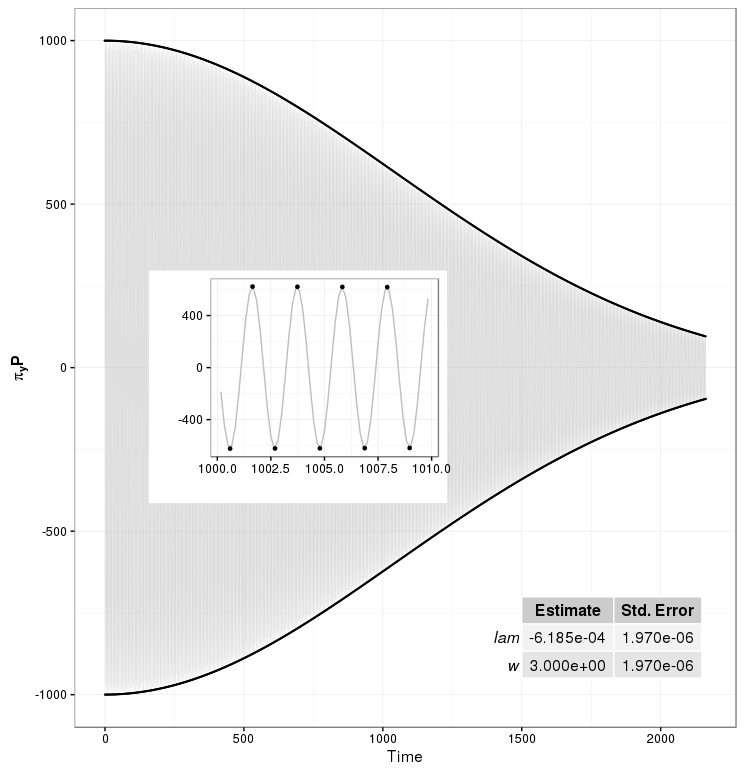
\includegraphics[scale=.5]{../img/Sgl_NormDistros}
		\caption{Signal in the case of a normally distributed oscillation frequency.}
	\end{subfigure}
	\caption{Normally distributed phase space variables.\label{fig:Sgl_cDyNorm}}
\end{figure}


\end{document}